\section{Theoretical Analysis}
\label{sec:analysis}


We started by analyzing the circuit using Kirchhoff's current law. It states that the algebraic sum of currents in a network of conductors meeting at a point is zero. It can be written as follows:

\begin{center}
\begin{equation}
\sum_{i=1} I_i=0
\label{current law}
\end{equation}
\end{center}
Where n is the total number of branches with currents flowing towards or away from the node.
One can then establish a relation between current and voltage using Ohm's Law:

\begin{center}
\begin{equation}
U=R\,I
\label{current law}
\end{equation}
\end{center}
Where U the potential difference, R the resistance, and I the current flowing through said segment. We now introduce the motion of electrical conductance, G, as the reciprocal of resistance. Therefore

\begin{center}
\begin{equation}
G_i=\frac{1}{R_1}
\label{current law}
\end{equation}
\end{center}

\subsection{Steady-state at t<0}

We are now ready to analyse the circuit presented in \ref{fig:circuit}. Focusing, first, on the configuration for $t<0$, one can see that the voltage source $V_s$ is time independent. Therefore, the capacitor will charge and the current that flows through it will go to 0. This is due to the isolating properties of the material between the capacitor's plates. With this in mind, we were able to write down a set of linear equations that allow us to compute the voltages in each node. We present said equations in matrix form bellow.
\begin{center}
\begin{equation*}
\begin{bmatrix}
0&     0 & 0 & 1 & 0 & 0 & 0 & 0\\
1&     0 & 0 & 0 & 0 & 0 & 0 & 0\\
G(1)&  -(G(1)+G(2)+G(3))&    G(2)&   0&   G(3)&          0&   0&   0\\
0&     -(G(2)+Kb)&           G(2)&    0&    Kb&          0&   0&   0\\
-G(1)&   G(1)&                0&      0&    G(4)         &0   &G(6)    &0\\
0&       0&                   0&      0&     1&          0&   Kd*G(6)&-  1\\
0&      -Kb&                  0&      0&    G(5)+Kb&    -G(5)&       0&       0\\
0&       0&                   0&       0&    0&           0&   -(G(6)+G(7))&    G(7)\\

\end{bmatrix}
 \begin{bmatrix} V_1\\V_2\\V_3\\V_4\\V_5\\V_6\\V_7\\V_8 \end{bmatrix} =
 \begin{bmatrix} 0\\V_s\\0\\0\\0\\0\\0\\0 \end{bmatrix}
\end{equation*}
\end{center}

Solving the system presented above, we obtained the following results for the voltages in each node.

\begin{table}[H]
  \centering
  \begin{tabular}{|l|r|}
    \hline
    {\bf Name} & {\bf Value [V]} \\ \hline
    \input{../mat/data_alinea_1}
  \end{tabular}
  \caption{Theoretical Values for VOLTAGES using Octave}
  \label{tab:alinea1_voltagens_tab}
\end{table}

%===============================================================
%alinea 2
%===============================================================
\subsection{Circuit at t=0}

We now want to obtain the equivalent resistance of the circuit as seen from the capacitor's terminals.
Thevenin’s Theorem states that it is possible to simplify any linear circuit to an equivalent circuit with just a single voltage source and a resistor ($R_{eq}$) in series with said voltage source.
To apply the Theorem, we start by excluding any independent voltage sources (in this case, $V_s$). Then, we substituted the element from which we wish to obtain the equivalent resistance, i.e. the capacitor, for a voltage source with voltage $V(6)-V(8)$, where V(6) and V(8) are the voltages in the capacitor's terminals. Let $I_x$ be the current flowing through this new voltage source, one can obtain the equivalent resistance as follows.

 \begin{center}
\begin{equation}
R_{eq}=\frac{V(6)-V(8)}{I_x}
\label{current law}
\end{equation}
\end{center}

We already know the value of $V(6)-V(8)$, so we only need to obtain the value of $I_x$. We do so by applying Kirchhoff's current law again, this time to a slightly different circuit (remember, $V_s$ was removed and the capacitor was replaced by an independent voltage source.). Most of the derived equations are similar or identic to the ones presented before, after all, we are working with circuits that are much alike. We choose to omit the voltage in node 4. This is known to be 0 once that it is connected to the ground.
\begin{equation*}
\begin{bmatrix}
  -(G(1)+G(2)+G(3))&  G(2) &  G(3)&        0&       0&        0&        0\\
  -(G(2)+Kb)&       G(2)&    Kb&           0&       0&         0&             0\\
 G(1)&          0&     G(4)&         0&      G(6)&           0&           0\\
  -Kb&                 0&     G(5)+Kb&      -G(5)&    0&     0&           -1\\
   0&       0&             1&           0&       Kd*G(6)&      -1               0\\
   0&       0&         0&          1&             0&             -1&       0\\
   0&      0&     0&           0&       -(G(6)+G(7))&       G(7)&      0\\



\end{bmatrix}
 \begin{bmatrix} V_1\\V_2\\V_3\\V_5\\V_6\\V_7\\V_8\\I_x \end{bmatrix} =
 \begin{bmatrix} 0 \\ 0 \\ 0 \\ 0 \\ 0 \\ V_6-V_8 \\ 0\end{bmatrix}
\end{equation*}

Once discovered the value for $R_eq$, we can calculate the capacitor's time constant, which is given by
 \begin{center}
\begin{equation}
\tau=C\,R_{eq}
\label{time_constant}
\end{equation}
\end{center}

Solving the system we obtained the following values for $R_eq$, $I_x$ ans $\tau$.

\begin{table}[H]
  \centering
  \begin{tabular}{|l|r|}
    \hline
    {\bf Name} & {\bf Value} \\ \hline
    \input{../mat/res_eq}
  \end{tabular}
  \caption{Equivalent Resistance}
  \label{tab:R_eq}
\end{table}

the voltages for the remaining nodes are as follows

\begin{table}[H]
  \centering
  \begin{tabular}{|l|r|}
    \hline
    {\bf Name} & {\bf Value V[V] and I[A]} \\ \hline
    \input{../mat/data_alinea_2}
  \end{tabular}
  \caption{Theoretical Values for VOLTAGES using Octave}
  \label{tab:alinea2_voltagens_tab}
\end{table}

This procedure is extremely useful because it allows us to transform the original circuit to a much simpler one. In fact, in order to study the behaviour of the capacitor as it charges and discharches (notice that until now we have considered the capacitor as being fully charged). It is the simplification of the problem that allow us to calculate the capacitor's time constant and from there obtain differential equations that we can actually solve.
Furthermore, it's important to state that this step is the analysis of the circuit at t=0, the instant in which the voltage source switches from being constant to being sinusoidal. Effectively, in this instant, $V_{s}=0$, and the only voltage that necessarily stays the same is the capacitor voltage, all the other ones may or may not change. That's also the reason why we've replaced the capacitor with a Voltage Source $V_{x}$. Not only that, but
this procedure is necessary for us to know the initial conditions for the natural solution of the voltage in node 6.
With this in mind, we are now going to study how the voltages in the capacitors terminals vary over time.

%==============================================================
%alínea 3
%==============================================================

\subsection{ Transient Analysis - Natural Solution for t$>$0}
We want to compute node 6's voltage with respect to time. First we need to compute its natural solution. Since we know the form of the explicit solution  (an exponential), we just the need to know the node 6's voltage at $t=0$ and at $t \to \infty $.
The latter is $0$ (the natural solution is the solution for a circuit that doesn't impose a voltage, i.e, doesn't have an independent voltage source, so naturally $V_{6}$ decays to $0$), and the former was calculated in the last section. However, we can say that
the initial condition for this case is, in reality, the capacitor's voltage ,$V_x$, at $t<0$, because it's this condition that dictates $V_6$ at $t=0$. The plot of the form


\begin{center}
\begin{equation}
V_{6n}(t)=V_6(0) e^{-\frac{1}{R_{eq}C}}
\label{ExplicitNaturalSolution}
\end{equation}
\end{center}
is shown below:

\begin{figure}[H]
  \centering
  \includegraphics[width=10cm]{natural.eps}
  \caption{Natural Solution for $V_{6}$}
  \label{fig:OctaveNaturalSolution}
\end{figure}

We see that the voltage decays exponentially.
%===============================================================
%alinea 4
%===============================================================
\subsection{Transient Analysis - Forced Solution}
We now want to compute the forced solution. We know that these explicit solutions (for the different nodes/components of the circuit) all oscillate in the same frequency as the independent voltage source. With this, one can make use of the complex notation to
simplify the problem. We can turn a differential equation into a Phasor relation, which is a complex number that can represent each node's voltage or component's current, and whose module and angle represent, respectively, their amplitude and oscillation's phase.
We then ran a nodal analysis using Phasor notation, and solved the following system:

\begin{equation*}
\begin{bmatrix}
   0 &      0 & 0 & 1 & 0 & 0 & 0 & 0\\
1 &      0 & 0 & 0 & 0 & 0 & 0 & 0\\
G(1) &   -(G(1)+G(2)+G(3)) &     G(2) &    0 &    G(3) &           0 &    0 &    0\\
0 &      -(G(2)+Kb) &            G(2) &     0 &     Kb &           0 &    0 &    0\\
-G(1) &    G(1) &                 0 &       0 &     G(4)          & 0    & G(6)     & 0\\
0 &        0 &                    0 &       0 &      1 &           0 &    Kd*G(6) &  -1\\
0 &        0 &                    0 &        0 &     0 &            0 &    -(G(6)+G(7)) &     G(7)\\
0 &        -Kb &                  0 &         0 &      G(5)+Kb &     -G(5)-Y &      0 &         Y\\

\end{bmatrix}
 \begin{bmatrix} \tilde{V_1}\\ \tilde{V_2}\\ \tilde{V_3}\\ \tilde{V_4}\\ \tilde{V_5}\\ \tilde{V_6}\\ \tilde{V_7} \\ \tilde{V_8} \end{bmatrix} =
 \begin{bmatrix} 0 \\ \tilde{V_s} \\ 0 \\ 0 \\ 0 \\0 \\ 0 \\ 0\end{bmatrix}
\end{equation*}
where Y is the inverse of the capacitor's impedance ("resistance" equivalent in complex form).
We got the following results:

\begin{table}[H]
  \centering
  \begin{tabular}{|l|r|}
    \hline
    {\bf Name} & {\bf Value} \\ \hline
    \input{../mat/data_alinea_d}
  \end{tabular}
  \caption{Phasors in each node}
  \label{tab:complex_phasors}
\end{table}

Thus, taking $\tilde{V_6}$'s magnitude and phase, we then plot the sinusoidal (forced) solution:

\begin{figure}[H]
  \centering
  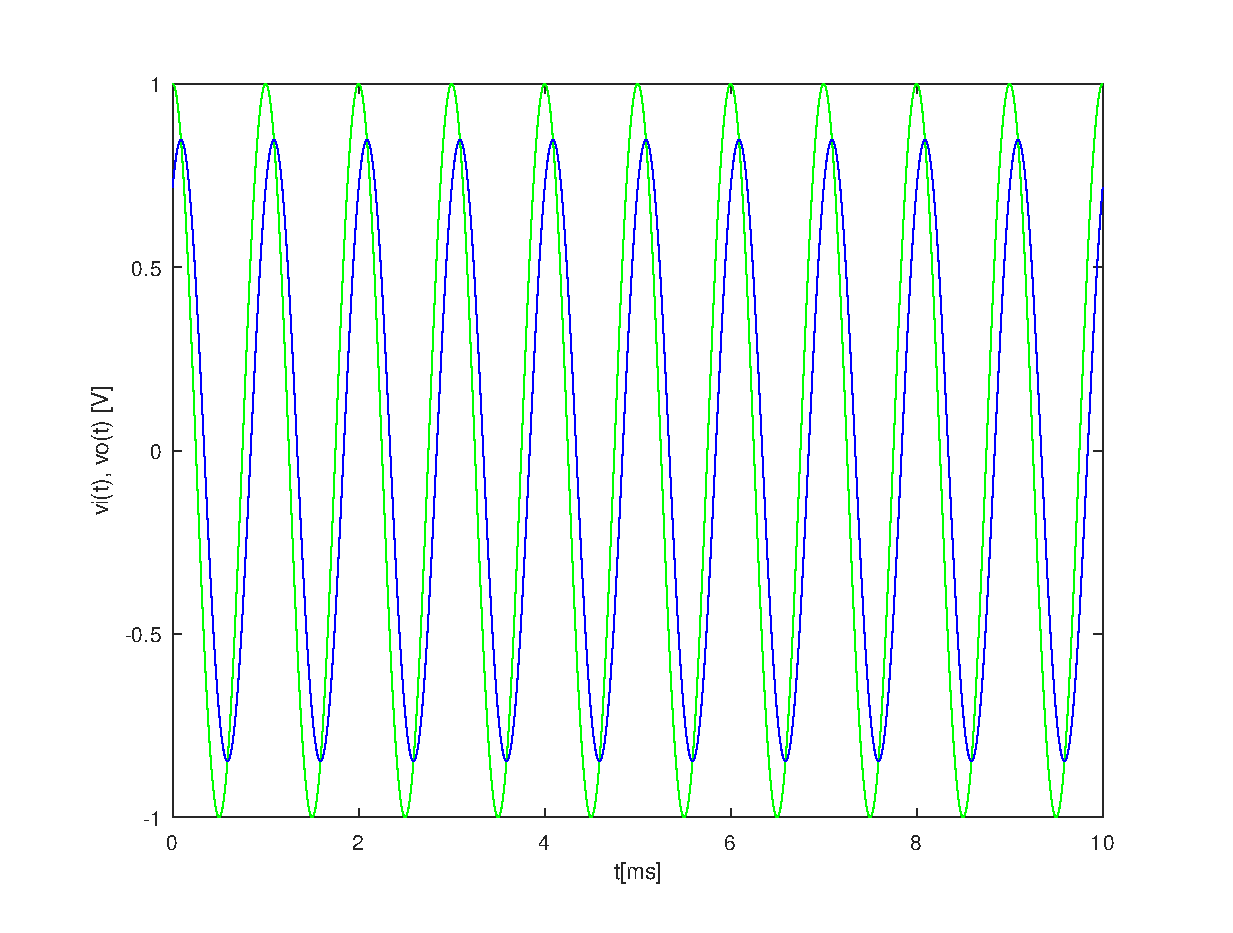
\includegraphics[width=10cm]{forced.eps}
  \caption{Forced Solution for $V_{6}$}
  \label{fig:OctaveForcedSolution}
\end{figure}

%=====================================
%alínea 5
%=====================================
\subsection{Transient Analysis - Final total solution}
Now we just add the natural and the forced solution to get $V_6(t)$. Plotting this alongside the independent voltage source we get:

\begin{figure}[H]
  \centering
  \includegraphics[width=10cm]{final.eps}
  \caption{$V_6(t)$ and $V_s(t)$}
  \label{fig:OctaveFinalSolution}
\end{figure}

Here we can clearly see that the natural solution dictates the initial time evolution, but the voltage quickly enters a steady-state, oscillating with the same frequency as $V_s$, but
with different amplitude and phase.

%===================================
%alínea 6
%===================================

\subsection{Frequency Analysis}

\section{alinea 6}
We want, now, to study how the frequency of the voltage independent source, $V_s$, may affect the voltages and phases in every other node.
We start by considering that the phase in $V_s$ is 0. We can always do that since the phase are always relative to each other. One can imagine a time translation so that this holds true every time.
Once obtained the imaginary amplitudes for the voltages in each node, it becomes trivial to find the real amplitude and phase shift.
Let $\mathcal{A}$ be the complex amplitude, $A$ the real amplitude, and $\phi$ the phase shift. We can write the following expressions

\begin{center}
    \begin{equation}
        A=\sqrt{Re^2(\mathcal{A})+Im^2(\mathcal{A})}=||\mathcal{A}||
    \end{equation}
\end{center}

\begin{center}
    \begin{equation}
        \phi=acrtan\left(\frac{Im(\mathcal{A})}{Re(\mathcal{A})}\right)=arg(\mathcal{A})
    \end{equation}
\end{center}

If we focus on the matrix \ref{eq:} we can see that if we remove the $6^{th}$ column and the last line, we can remove the $6^{th}$ unknown variable. Notice that if this is done we are left with a matrix that is frequency independent. This means that all of the other variables must by frequency independent.

We have computed the complex amplitudes for a very large finite set frequencies, ranging from 0.1 Hz to 1 MHz. We now present the obtained values for the phase shift of $V_6$, $V_8$, $V_c$ and $V_s$. Notice that $V_s$ is imposed to have null phase and amplitude of 1.

\begin{center}
    \includegraphics[scale=0.5]{alinea_6_amp}
    \captionof{figure}{Amplitude as a function of frequency}
     \label{fig:amp(f)1}
\end{center}

\begin{center}
    \includegraphics[scale=0.5]{alinea_6_amp_2}
    \captionof{figure}{Amplitude as a function of frequency}
     \label{fig:amp(f)2}
\end{center}

We chose to create two different plots, only one of which contains the difference in amplitudes. We did so since, as the frequency goes to infinity $V_C\longrightarrow0$, this makes it more difficult to understand what it happening on a bigger scale.
As expected, we can see that $V_8$ is frequency independent. Also as theoretically predicted, the voltage difference between the capacitors terminals goes to 0 too, once that the impedance is inversely proportional to the frequency. The voltage difference is itself proportional to the impedance.

Plotting the same results for the phase shifts we get
\begin{center}
    \includegraphics[scale=0.5]{alinea_6_fases}
    \captionof{figure}{Amplitude as a function of frequency}
     \label{fig:amp(f)1}
\end{center}

As predicted, $V_s$'s phase remains, by construction, 0, and $V_8$'s remains constant, as expected.
